\documentclass{standalone}

\usepackage[latin1]{inputenc}
\usepackage{amsmath}
\usepackage{amssymb}
\usepackage{amsthm}

\usepackage{tikz}

%% generates a tightly fitting border around the work
%\usepackage[active,tightpage]{preview}
%\PreviewEnvironment{tikzpicture}
%\setlength\PreviewBorder{0.5mm}
%%\renewcommand\PreviewBbAdjust{-\PreviewBorder 1mm -1.15mm -0.85mm}

\usepackage{color}

%\pagestyle{empty}

\begin{document}

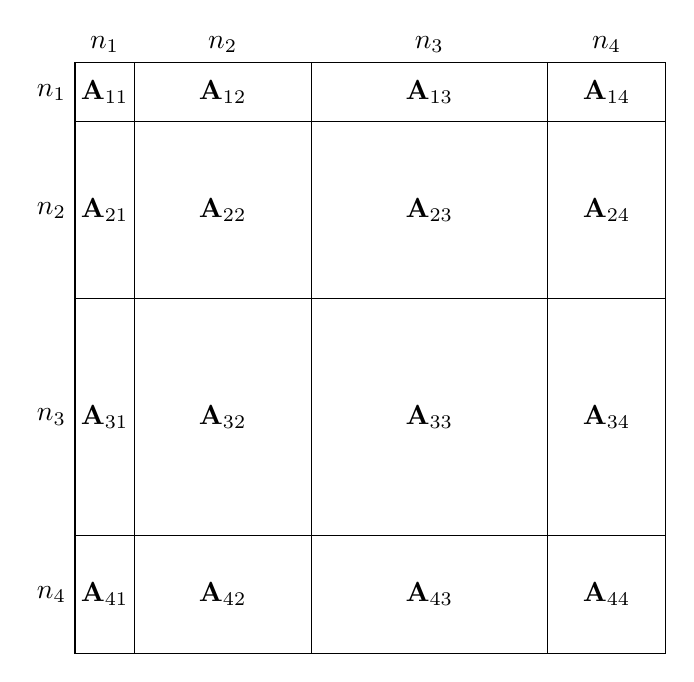
\begin{tikzpicture}[scale=0.75, auto]
  \draw (0.5,11.3) node{$n_{1}$};
  \draw (2.5,11.3) node{$n_{2}$};
  \draw (6,11.3) node{$n_{3}$};
  \draw (9,11.3) node{$n_{4}$};
  \draw (-0.4,10.5) node{$n_{1}$};
  \draw (-0.4,8.5) node{$n_{2}$};
  \draw (-0.4,5) node{$n_{3}$};
  \draw (-0.4,2) node{$n_{4}$};
  % the first row
  \draw (0.5,10.5) node{$\mathbf{A}_{11}$};
  \draw (0,10) rectangle ++(1,1);
  \draw (2.5,10.5) node{$\mathbf{A}_{12}$};
  \draw (1,10) rectangle ++(3,1);
  \draw (6,10.5) node{$\mathbf{A}_{13}$};
  \draw (4,10) rectangle ++(4,1);
  \draw (9,10.5) node{$\mathbf{A}_{14}$};
  \draw (8,10) rectangle ++(2,1);
  % the second row
  \draw (0.5,8.5) node{$\mathbf{A}_{21}$};
  \draw (0,7) rectangle ++(1,3);
  \draw (2.5,8.5) node{$\mathbf{A}_{22}$};
  \draw (1,7) rectangle ++(3,3);
  \draw (6,8.5) node{$\mathbf{A}_{23}$};
  \draw (4,7) rectangle ++(4,3);
  \draw (9,8.5) node{$\mathbf{A}_{24}$};
  \draw (8,7) rectangle ++(2,3);
  % the third row
  \draw (0.5,5) node{$\mathbf{A}_{31}$};
  \draw (0,3) rectangle ++(1,4);
  \draw (2.5,5) node{$\mathbf{A}_{32}$};
  \draw (1,3) rectangle ++(3,4);
  \draw (6,5) node{$\mathbf{A}_{33}$};
  \draw (4,3) rectangle ++(4,4);
  \draw (9,5) node{$\mathbf{A}_{34}$};
  \draw (8,3) rectangle ++(2,4);
  % the fourth row
  \draw (0.5,2) node{$\mathbf{A}_{41}$};
  \draw (0,1) rectangle ++(1,2);
  \draw (2.5,2) node{$\mathbf{A}_{42}$};
  \draw (1,1) rectangle ++(3,2);
  \draw (6,2) node{$\mathbf{A}_{43}$};
  \draw (4,1) rectangle ++(4,2);
  \draw (9,2) node{$\mathbf{A}_{44}$};
  \draw (8,1) rectangle ++(2,2);
\end{tikzpicture}

\end{document}
